\chapter[Methods]{Methods} \label{ch:methods}

At a high level, the goal of any quantum circuit optimization is to reduce the complexity of the input circuit.
A core assumption of circuit optimization in the ZX-calculus is that ZX-diagrams with fewer spiders typically correspond to simpler circuits.
Earlier, however, we noted that local changes (e.g., connectivity) in a ZX-diagram can drastically affect the complexity of the associated circuit obtained via extraction.
However, no existing optimization procedure over ZX-diagrams addresses this and searches this local space.
The \codeword{full_reduce} method described in Section \ref{sec:zx-circ-opt} is the quintessential example of this lost opportunity.
After the two simplification rules can no longer be applied, the final circuit is taken to be that which is extracted from the resulting simplified ZX-diagram;
however, there may be an equivalent ZX-diagram lurking nearby whose associated circuit is markedly less complex.

In this thesis, we explore the utility of searching this local space of equivalent ZX-diagrams.
To do so, we first need rewrite rules that modify a ZX-diagram in a manner other than spider removal that may reduce circuit complexity.
Indeed, a rule that introduces several additional spiders alongside changes in connectivity may in turn yield a less complex circuit.
We refer to these rewrite rules as \emph{congruences}.
Given a set of congruences, we then need a procedure to search the space of equivalent ZX-diagrams generated by an input ZX-diagram and these rules.
We can then devise strategies for incorporating this local search into existing methods for circuit optimization in the ZX-calculus.

We present the methods of our work in this order.
First, we generalize the original (non-simplification) variants of local complementation and pivoting to ZX-diagrams with arbitrary phases.
We then describe two search procedures, simulated annealing (SA) and genetic algorithms (GA).
% for searching the space of ZX-diagrams generated by these congruences.
We also define a measure of circuit complexity and discuss candidate objective functions to guide search. % to the ZX-diagram whose circuit has minimal complexity.
Lastly, we discuss how this search can be incorporated into existing optimization pipelines.
% Our primary strategy is to first simplify a ZX-diagram using existing methods and subsequently search the local variants of the simplified ZX-diagram.
% Alternatively, we can use SA or GA as the principal means of optimization.
% In this more ambitious approach, congruences can be combined with simplification rules to form an action set over which search is applied.

\section{Congruences}\label{sec:congruences}

The non-simplification versions of local complementation and pivoting presented in Section \ref{sec:zx-circ-opt} embody the desired properties of congruences.
They change the connectivity of the ZX-diagram without introducing an unwieldy number of additional gates, presenting an opportunity for a potential reduction in circuit complexity.
However, Equations \ref{eq:gs-local-comp} and \ref{eq:gs-pivot} only apply to spiders with zero phase and a single wire.

% Useful for spacing:
% https://tex.stackexchange.com/questions/54587/vertical-spacing-within-align-environment-accounting-for-fractions
We can apply the rules of the ZX-calculus and Equation \ref{eq:gs-local-comp} to generalize local complementation to arbitrary phases ($\alpha_i, \beta_i \in [0, 2 \pi)$):
% note: can do \tag{\theequation} to get a number
% {\allowdisplaybreaks
\begin{spreadlines}{0.8em}% tweak
  \begin{align*}
    \tikzfig{gen-lc-single/0} &\stackrel{(\bm f)}{=} \tikzfig{gen-lc-single/1} \\
    &\stackrel{(\ref{eq:gs-local-comp})}{=} \tikzfig{gen-lc-single/2} \\
    &\stackrel{(\bm i1)}{=} \tikzfig{gen-lc-single/3} \\
    &\stackrel{(\bm f)}{=} \tikzfig{gen-lc-single/4} \\
    &\stackrel{(\bm f)}{=} \tikzfig{gen-lc-single/5} \\[0.8em]
    &\stackrel{(\ref{eq:had-short})}{=} \tikzfig{gen-lc-single/6}\stepcounter{equation}\tag{\theequation}\label{eq:gen-phase-lc}
  \end{align*}
\end{spreadlines}
% }
Equation \ref{eq:gen-phase-lc} can be easily extended to apply for an arbitrary number of wires connected to each spider:
% {\allowdisplaybreaks
\begin{spreadlines}{0.8em}% tweak
  \begin{align*}
    \tikzfig{gen-lc-mul/0} &\stackrel{(\bm f)}{=} \tikzfig{gen-lc-mul/1} \\
    &\stackrel{(\ref{eq:gen-phase-lc})}{=} \tikzfig{gen-lc-mul/2} \\
    &\stackrel{(\bm f)}{=} \tikzfig{gen-lc-mul/3}\stepcounter{equation}\tag{C1}\label{eq:gen-io-lc}
  \end{align*}
\end{spreadlines}
% }
% Equation \ref{eq:gs-pivot}:
Similarly, we can generalize pivoting to arbitrary phases:
% {\allowdisplaybreaks
\begin{spreadlines}{0.8em}% tweak
  \begin{align*}
    \tikzfig{gen-pivot-single/0} &\stackrel{(\bm f)}{=} \tikzfig{gen-pivot-single/1} \\
    &\stackrel{(\ref{eq:gs-pivot})}{=} \tikzfig{gen-pivot-single/2} \\
    &\stackrel{(\bm f)}{=} \tikzfig{gen-pivot-single/3}\stepcounter{equation}\tag{\theequation}\label{eq:gen-phase-pivot}
  \end{align*}
\end{spreadlines}
% }
Again, we can extend this rewrite rule for arbitrary wiring:
\begin{spreadlines}{0.8em}% tweak
  \begin{align*}
    \tikzfig{gen-pivot-mul/0} &\stackrel{(\bm f)}{=} \tikzfig{gen-pivot-mul/1} \\
    &\stackrel{(\ref{eq:gen-phase-pivot})}{=} \tikzfig{gen-pivot-mul/2} \\
    &\stackrel{(\bm f)}{=} \tikzfig{gen-pivot-mul/3}\stepcounter{equation}\tag{C2}\label{eq:gen-io-pivot}
  \end{align*}
\end{spreadlines}
% Equations \ref{eq:gen-io-lc} and \ref{eq:gen-io-pivot} will serve as our primary congruences -- those rewrite rules that, when applied, maintain a similar graph complexity but potentially reduce the circuit complexity.
Equations \ref{eq:gen-io-lc} and \ref{eq:gen-io-pivot} will serve as our primary congruences because they maintain a similar graph complexity (e.g., number of spiders and wires) but, due to their effects on connectivity, can produce circuits of varying complexities.
Equation \ref{eq:gen-io-lc} can be applied to any spider with a degree of more than 1.
Equation \ref{eq:gen-io-pivot} can be applied to any pair of connected spiders.


\section{Search Procedures}

The space of ZX-diagrams generated by an input ZX-diagram and these congruences is combinatorial and therefore cannot be searched exhaustively.
We can instead formulate this search as an optimization problem where the set of isomorphic ZX-diagrams are the states (reachable by congruence applications) that are evaluated by some quantitative measure of circuit complexity.
Here we describe two search procedures as well as several candidate objective functions that either measure circuit complexity directly or use ZX-diagrammatic properties as a proxy.

\subsection{Simulated Annealing}\label{sec:sa}

Simulated annealing is an optimization technique named after the annealing process in metallurgy in which a molten hot metal is cooled in a slow, controlled fashion in order for it to reach its most stable form.
In SA, this notion of slow cooling is interpreted as a slow decrease in the probability of accepting worse solutions.
In this way, the algorithm initially explores a broad region of the the search space and progressively narrows its scope.

More formally, the SA algorithm maintains a current state $s$ and at each step randomly considers some neighboring state $s^*$.
The algorithm then chooses whether or not to replace $s$ with $s^*$ via a Bernoulli random variable parameterized by the \emph{acceptance probability}, denoted $P(s, s^*, T)$. % FIXME: wrong subject for "denoted"?
The acceptance probability depends on (1) the \emph{energy} (i.e., objective) \emph{function}, and (2) the \emph{temperature}.
The energy function $E(s)$ assigns a score to each state (lower is better).
If $E(s') < E(s)$, then $s$ is always replaced with $s^*$ (i.e., $P(s, s^*, T) = 1$).
Otherwise, $P(s, s^*, T) = exp(-\frac{E(s^*) - E(s)}{T})$ where the temperature $T$ controls the likelihood of moving to a higher energy state.
Note that $P(s, s^*, T)$ is inversely proportional to $E(s^*) - E(s)$ and directly proportional to $T$.
Informally, this means that $s^*$ is more likely to be accepted if it is closer in energy to $s$ and with a higher temperature.
$T$ is initialized to some positive value and progressively decreases to zero.
At each step, $T$ is updated as $T = T * c$ where $c \in [0, 1)$ is the \emph{cooling} parameter. % FIXME: Change in code to always cool, not just when a change is made.
In this way, SA converges towards a greedy algorithm and is more likely to accept $s^*$ when $E(s^*) > E(s)$ early in search when $T$ is high.
The algorithm terminates when a maximum number of steps $k_{max}$ is reached (default: $k_{max} = 1000$).
Algorithm \ref{alg:sa} provides an overview of this procedure.

\begin{algorithm}[t]
  \caption{Simulated annealing
    \label{alg:sa}}
  \begin{algorithmic}[1]
    % \Require{$x$ and $y$ are packed \DNA{} strings of equal length $n$}
    % \Statex
    \Function{SimAnneal}{$s_0, T, c, k_{max}$}
      % \Let{$z$}{$x \oplus y$} \Comment{$\oplus$: bitwise exclusive-or}
      \Let{$s$}{$s_0$}
      \For{$i \gets 0 \textrm{ to } k_{max}$}
        \Let{$s^*$}{randomly sampled neighbor of $s$}
        \If{$E(s^*) < E(s)$ {\bf or} $\text{random}(0, 1) < exp(-\frac{E(s^*) - E(s)}{T})$}
          \Let{$s$}{$s^*$}
        \EndIf
        \Let{$T$}{$T * c$}
      \EndFor
      \State \Return{$s$}
    \EndFunction
  \end{algorithmic}
\end{algorithm}

In this work, the state is a ZX-diagram and neighbors are sampled via the probabilistic application of rewrite rules.
For example, to anneal using the rewrite rules described in Section \ref{sec:congruences}, $s^*$ would be sampled by first choosing one of Equation \ref{eq:gen-io-lc} or Equation \ref{eq:gen-io-pivot} and then choosing a spider or pair of connected spiders to which the rule will be applied.
Note that we use Equations \ref{eq:gen-io-lc} and \ref{eq:gen-io-pivot} by default but in theory any set of rewrite rules can be used.

\subsection{Genetic Algorithms}

Genetic algorithms are a class of optimization procedures inspired by the process of natural selection.
Rather than maintaining a single state (e.g., as in SA), a \emph{population} of candidate solutions is \emph{evolved}.
This evolution is guided by a \emph{fitness function} and operates via biologically inspired notions of \emph{mutation}, \emph{crossover}, and \emph{selection}.
In this work, we define fitness such that lower fitness is better to remain consistent with the energy function described in Section \ref{sec:sa}.
% For details on objective functions used to guide circuit optimization, see Section \ref{sec:obj-funcs}.

A genetic algorithm operates in the following general fashion.
First, a population of candidate solutions (i.e., \emph{mutants}) is randomly generated.
The population size is typically fixed to some $n_{mutants}$.
This initial population then evolves in a series of \emph{generations}.
Each generation consists of two parts: (1) selection and (2) application of genetic operators (e.g., mutation and crossover).
In the selection step, a score is assigned to each mutant via the fitness function and a new population is chosen given these scores.
For example, a naive selection method would set the population to $n_{mutants}$ copies of the best-scoring mutant.
Given this surviving population, the second step involves applying genetic operators to obtain a revised, diverse population.
The two most common genetic operators are mutation and crossover.
Analogous to mistakes being made during replication of a DNA sequence, a mutation operator involves randomly tweaking a single mutant.
In the case where mutants are represented as bit strings, the canonical example of a mutation operator is a bit-flip.
Alternatively, a crossover operator produces a new mutant given two or more existing mutants;
this is analogous to reproduction and biological crossover.
For example, given two mutants represented as strings, a new mutant can be generated by swapping the two segments defined by a random position.
Evolution proceeds for $n_{gens}$ generations and the algorithm returns the mutant with the highest fitness throughout search.
This process is summarized in Figure \ref{fig:ga}.

\begin{figure}
\centering
\tikzfig{ga}
\caption{An overview of genetic algorithms.}
\label{fig:ga}
\end{figure}

% \ctikzfig{ga}

\iffalse
\begin{figure}[t]
\centering
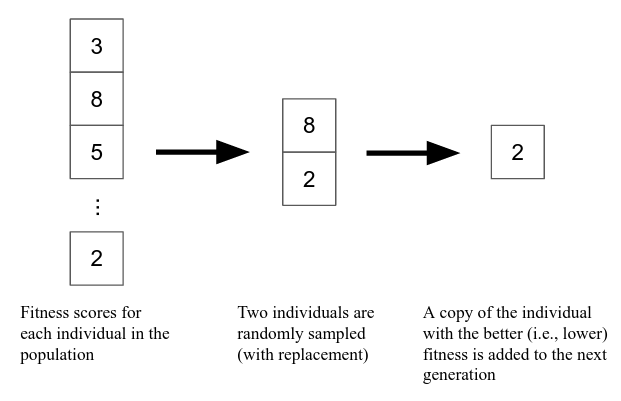
\includegraphics[width=8cm]{img/tournament.png}
\caption{An overview of the simple variant of tournament selection used in this work.
  Two mutants are randomly chosen and the winner with better fitness is selected.}
\label{fig:tourn}
\end{figure}
\fi

The default in this work is to represent mutants as ZX-diagrams and to use rewrite rules as mutation operators.
As is common in practical applications of genetic algorithms, we do not use any crossover operators though this is an attractive area for future exploration given the graphical nature of ZX-diagrams. % FIXME: cite
Lastly, we use \emph{tournament selection} to determine the surviving mutants at each generation.
In this selection method, $k_{tourn}$ mutants are selected to compete in a ``tournament'' from which a winner is chosen based on fitness.
This is repeated $n_{mutants}$ times with replacement to obtain a surviving population.
We use a simple variant of tournament selection in which $k_{tourn} = 2$ and the winner is simply the mutant with better (i.e., lower) fitness.


\subsection{Objective Functions}\label{sec:obj-funcs}

% look up ion trap papers, single qubit gates with 99.9 fidelity and two qubit with 99 fidelity. 10 perc difference in fidelity. chris ballance

Both the energy function (used in SA) and the fitness function (used in GA) are instances of an \emph{objective function}.
An objective function measures the ``goodness'' of a particular solution to an optimization problem.
For our purposes, we require an objective function that, given a ZX-diagram, provides a reasonable measure of the complexity of the circuit obtained via extraction.
For consistency, all objective functions are defined in such a way that a low score is better (i.e., a low score indicates low complexity).

The most straightforward objective function involves extracting a circuit and measuring its complexity directly.
A quantitative measure of circuit complexit is also useful for evaluating our optimization techniques.
Given a circuit $C$ in terms of single- and 2-qubit gates, we define its complexity $Comp(C)$ to be a weighted average of its single-qubit and 2-qubit gate counts:
\begin{align*}
  Comp(C) = 10 * (\text{\# 2-qubit gates}) + 1 * (\text{\# single-qubit gates})
\end{align*}
A scaling factor of 10 is chosen because 2-qubit gates are typically an order of magnitude more costly to implement than a single-qubit gate~\cite{campbell2017roads, ballance2016high}.
Note that \codeword{basic_optimization} is always applied to the extracted circuit.

% There are two possible high-level approaches to scoring: (1) extract the circuit and measure its complexity directly, or (2) measure some property of the ZX-diagram that is a reasonable proxy for the complexity of the associated circuit.
% Even if (1) is not used to guide search, we still require a quantitative measure of circuit complexity to analyze both our optimization methods and the estimates provided by some instance of (2).

However, extracting a circuit from the ZX-diagram every time we want to measure its complexity is costly.
For example, evolving a population of 50 mutants for 100 generations would require 5000 extractions.
Instead, we could measure some property of the ZX-diagram that is a reasonable proxy for $Comp(C)$ (where $C$ is the circuit obtained via extraction).
The following are candidate properties to serve as such a proxy:
% Instead, the following are several quantities of a ZX-diagram that may serve as reliable proxies for $Comp(C)$ (where $C$ is the circuit obtained via extraction):
\begin{itemize}
\item
  The number of edges
\item
  The density of the underlying graph
\item
  The centrality of the underlying graph
\end{itemize}
The ZX-diagram is assumed to be graph-like.

Measuring the ZX-diagram is clearly preferable but relies on the existence of a property that is sufficiently correlated to $Comp$.
Note that none of the above objective functions, including $Comp$, are normalized and therefore scores can only be compared between isomorphic ZX-diagrams.

\section{Circuit Optimization Strategies}

Here we describe how we use these congruences and search procedures for quantum circuit optimization.
We first outline our primary method which involves first applying off-the-shelf methods to obtain a simplified ZX-diagram and subsequently searching the space of equivalent ZX-diagrams generated by Equations \ref{eq:gen-io-lc} and \ref{eq:gen-io-pivot}.
We then describe an alternative, more general approach in which Equations \ref{eq:gen-io-lc} and \ref{eq:gen-io-pivot} are combined with simplification rules to form a single action set over which search is applied.


\begin{figure}[t]
\centering
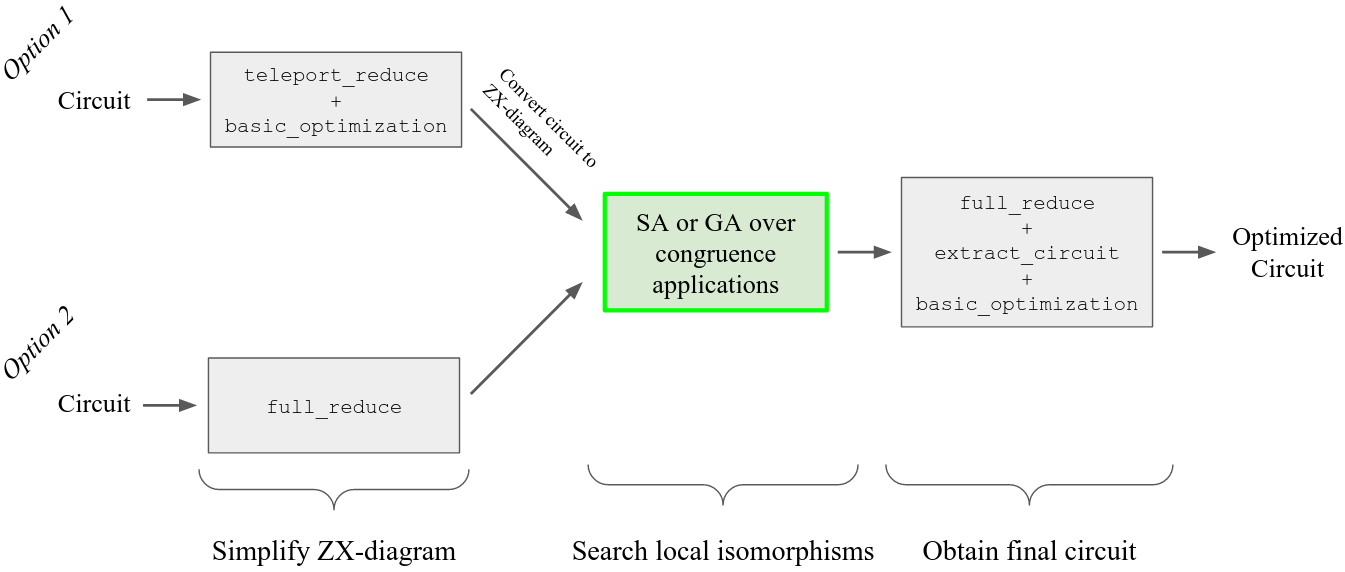
\includegraphics[width=15cm]{img/primary-overview.png}
\caption{
  An overview of our primary optimization strategy.
  Given an input circuit, a simplified ZX-diagram is obtained via one of two off-the-shelf methods.
  Then, we search for an equivalent ZX-diagram with similar graph complexity but lower circuit complexity (highlighted in green).
  A circuit is extracted from the final ZX-diagram and standard circuit-level optimizations are performed.
}
\label{fig:primary}
\end{figure}

\subsection{Primary: Post-Simplification Search}\label{sec:primary}

% changed from "the TR and FR pipelines described in Section ..."
Our primary optimization strategy improves upon the two pipelines described in Section \ref{sec:zx-circ-opt} by searching local variants of the simplified ZX-diagrams.
Given an input circuit, we can obtain a simplified ZX-diagram to seed search in one of two ways.
Firstly, we can apply \codeword{full_reduce}.
Importantly, we do not apply the entire \codeword{full_reduce} + \codeword{extract_circuit} + \codeword{basic_optimization} pipeline and convert the simplified circuit to a ZX-diagram as the complexity cost incurred by extraction will likely outweigh any simplifications achieved at the circuit-level.
Alternatively, since \codeword{teleport_reduce} short-circuits circuit extraction, we can apply \codeword{teleport_reduce} + \codeword{basic_optimization} and convert the simplified circuit to a ZX-diagram.
Given a simplified ZX-diagram, we can then apply SA or GA to search the space of ZX-diagrams generated by Equations \ref{eq:gen-io-lc} and \ref{eq:gen-io-pivot} for an equivalent ZX-diagram whose extracted circuit is less complex.
Note that search proceeds by first randomly selecting one of Equations \ref{eq:gen-io-lc} and \ref{eq:gen-io-pivot} and then randomly selecting a subject (i.e., spider or pair of connected spiders) for the selected congruence.
We denote the probability of selecting Equations \ref{eq:gen-io-lc} and \ref{eq:gen-io-pivot} as $p_{LC}$ and $p_{pivot}$, respectively (default: $p_{LC} = p_{pivot} = 0.5$).
An overview of this strategy is depicted in Figure \ref{fig:primary}.
% Note: Could alternatively have the "cloud" figure with graph complexity vs circuit complexity.

Since Equations \ref{eq:gen-io-lc} and \ref{eq:gen-io-pivot} break the circuit structure of a graph, it is reasonable to apply \codeword{full_reduce} because a circuit has to be extracted regardless.
Therefore, the default objective function scores a ZX-diagram by first applying \codeword{full_reduce}, extracting a circuit $C$ and applying simple circuit-level optimizations with \codeword{basic_optimization}, and measuring its complexity $Comp(C)$.
We can also apply \codeword{full_reduce} probabilistically via some free parameter $p_{fr}$ throughout search (default: $p_{fr} = 0.1$).
In SA, \codeword{full_reduce} is applied to the current state at each step with probability $p_{fr}$ while in GA \codeword{full_reduce} is applied to each mutant in a given generation with probability $p_{fr}$.

There are several opportunities to refine this strategy.
One example is applying Equations \ref{eq:gen-io-lc} and \ref{eq:gen-io-pivot} with unequal probabilities.
This could be beneficial if one congruence more effectively navigates the search space than the other.
Another possible refinement is non-uniform sampling of spiders (resp. pairs of spiders) to which Equation \ref{eq:gen-io-lc} (resp. Equation \ref{eq:gen-io-pivot}) will be applied.
The following are possible spider metrics to weight sampling for application of Equation \ref{eq:gen-io-lc}:
\begin{itemize}
\item
  Degree
\item
  Centrality (e.g., betweenness, Katz)
\item
  Total degree of neighbors
\end{itemize}
Similarly, the following are possible metrics to weight sampling of pairs of nodes for Equation \ref{eq:gen-io-pivot}:
\begin{itemize}
\item
  Sum of spider-wise metrics (e.g., total degree of the union of all neighbors)
\item
  Edge centrality (e.g., load, betweenness)
\item
  Edge dispersion
\end{itemize}
Lastly, we can experiment with different values of $p_{fr}$.


\subsection{Alternative: Congruences as First-Class Citizens}

An underlying assumption of \codeword{full_reduce} is that simplifying the ZX-diagram as much as possible is optimal.
However, removing spiders to fixpoint may come at a cost.
For example, later-stage spider removals may induce connectivity properties in the ZX-diagram (e.g., high-degree spiders, high density) that translate to a high 2-qubit count upon extraction.

To test this, we employ an alternative simplification strategy in which congruences are applied alongside simplifications rather than after the ZX-diagram is fully simplified.
More specifically, we treat individual simplification rules as actions and combine these with Equations \ref{eq:gen-io-lc} and \ref{eq:gen-io-pivot} to form a master action set.
These individual simplifications are the following: \textcolor{red}{FIXME itemize, and then a sentence on what they can be applied to}.
Given an input circuit, we convert it to a ZX-diagram and search over this master action set.
For search, we only use GA as maintaining a population of mutants rather than a single state (as in SA) is well-suited for the significantly higher branching factor.

\textcolor{red}{FIXME: If have time and space, can extend to the case where the state of GA is both circuit + ZX-diagram so that we can apply non-PyZX simplifications.}

% because going to fixpoint might be bad. go global instead. use all. congruences as first-class citizens
% Only use GA for this because handles branching factor better. can repr states as pairs so we can do non-pyzx optimizations! mutation operators take in pair and return apir. in practice, this owrks in one of two ways.





% only use GA as branching factor is too big

% Maybe simplifying to fixpoint isn't optimal, and introduces too many edges that lead to CNOTs to get us marginal T-count gain. So, we can just be careful right from the beginning!

% subsection: from scratch. just include congruences as a possible action along with all the others
% In this work, mutants are represented as pairs of ZX-diagrams and their associated circuits by default.
% This allows for mutation to occur at either the graph- or circuit-level.
% If a mutant is modified at the graph-level (i.e., via a rewrite rule), the associated circuit is obtained via extraction.
% Alternatively, traditional circuit-level optimizations can be applied and the correpsonding ZX-diagram can be generated directly from the modified circuit..
% mutation operator takes in a pair and returns a pair.

% (archived) -- FIXME: Other, more general combinations (e.g., GA with all simps, or search with other ``safe'' procedures).
